\documentclass[conference]{IEEEtran}
\IEEEoverridecommandlockouts

\usepackage[T1]{fontenc}
\usepackage{cite}
\usepackage{amsmath,amssymb,amsfonts}
\usepackage{graphicx}
\usepackage{booktabs}
\usepackage{multirow}
\usepackage{array}
\newcolumntype{L}[1]{>{\raggedright\arraybackslash}p{#1}}
\usepackage{algorithm}
\usepackage{algpseudocode}
\usepackage{xcolor}
\usepackage{tikz}
\usetikzlibrary{arrows.meta,positioning,fit,calc,shapes.geometric}
\usepackage[hidelinks]{hyperref}
\usepackage{url}

\newcommand{\paperval}{$^{*}$}            % value taken from the original paper
\renewcommand{\arraystretch}{1.08}
\setlength{\tabcolsep}{3.2pt}

\begin{document}

\title{XDA-IDS: An Explainable, Drift-Aware Lightweight Intrusion Detection System for IoT/IIoT Networks Using SHAP-Attribution Monitoring}

\author{
\IEEEauthorblockN{Muhammad Azmat}
\IEEEauthorblockA{\textit{Department of Data Science} \\
\textit{FAST School of Computing, National University of}\\
\textit{Computer and Emerging Sciences (FAST-NUCES)}\\
Islamabad, Pakistan \\
muhammadazmat018@gmail.com}
\and
\IEEEauthorblockN{Abdullah Ilyas}
\IEEEauthorblockA{\textit{Department of Data Science} \\
\textit{FAST School of Computing, National University of}\\
\textit{Computer and Emerging Sciences (FAST-NUCES)}\\
Islamabad, Pakistan \\
abdullahilyas436@gmail.com}
}

\maketitle

% ============================================================== ABSTRACT
\begin{abstract}
Lightweight deep-learning intrusion detection systems (IDS) for the Internet of Things (IoT) report high benchmark accuracy, but they are evaluated as static snapshots, miss rare attack families, and use explanations only after the fact. This paper presents XDA-IDS, which extends an explainable one-dimensional convolutional neural network (1D-CNN) IDS with three components: a class-balanced focal loss with frequency-encoded protocol fields, a label-free drift monitor that compares the SHAP attributions of each traffic window with a reference profile, and a retraining loop triggered by the monitor. XDA-IDS is evaluated on UNSW-NB15, WUSTL-IIoT-2021 and CICIoT2023 under a leak-free protocol, with unseen-attack-family streams, four injected drift types and cross-dataset transfer. A leakage audit shows that the base paper's protocol inflates UNSW-NB15 binary Macro-F1 from 0.899 to 0.985. Against the re-implemented leak-free base CNN, XDA-IDS raises UNSW-NB15 multiclass Macro-F1 from 0.356 to 0.409 (+14.9\% relative) and lifts Worms, Analysis and Shellcode recall from 0 to 0.88, 0.80 and 0.45, at 0.24\,ms per flow and 0.17\,M parameters; its false-positive rate, however, rises from 0.145 to 0.264. The SHAP-based monitor detects 11 of 11 drift and unseen-attack scenarios without labels, against 10 for an input Kolmogorov--Smirnov monitor and 6 for ADWIN; its KS-only variant keeps a 0.009 false-alarm rate. XGBoost remains the most accurate detector (Macro-F1 0.584). The results show that explanations can serve as an operational, label-free drift signal for edge IDS, while false positives and drift-type diagnosis remain open problems.
\end{abstract}

\begin{IEEEkeywords}
Intrusion detection, Internet of Things, concept drift, explainable AI, SHAP, class imbalance
\end{IEEEkeywords}

% ============================================================== INTRODUCTION
\section{Introduction}
IoT and Industrial IoT (IIoT) networks connect large numbers of resource-constrained devices whose traffic changes as firmware is updated, devices are added and attackers adopt new tools. Network intrusion detection systems (IDS) placed at IoT gateways must therefore classify flows in real time on limited hardware, remain reliable as traffic evolves, and give analysts reasons they can act on.

Recent lightweight deep-learning IDS address part of this problem. The base paper of this work, Udurume \textit{et al.}~\cite{udurume2026}, combines a compact 1D-CNN with SHAP explanations~\cite{lundberg2017} and reports F1-scores of 97.5\% and 94.0\% on UNSW-NB15 binary and multiclass tasks~\cite{moustafa2015}. Related studies add self-attention~\cite{sharma2025}, recurrent attention models tuned by metaheuristics~\cite{nasir2026,guo2026} and hybrid CNN--LSTM ensembles~\cite{chen2026}. Three limitations recur across this literature. First, models are trained once and tested on random splits in which every test attack also appears in training, so the effect of drift or new attack families is unknown. Second, explanations are descriptive: they are computed offline for interpretation or feature pruning and are never used while the model is deployed. Third, aggregate metrics hide rare-class failure; the base paper's own confusion matrix shows zero recall for Backdoor, Shellcode and Worms. Drift-aware IDS exist~\cite{obaidat2026,aly2025,agbedanu2025}, but they monitor raw inputs or labelled error rates and cannot explain what changed in the model's reasoning.

\textit{Research gap.} No existing lightweight IoT IDS uses its own explanations to detect, without labels, when it has become outdated or faces an unseen attack, while also explaining the change and maintaining detection of rare attacks.

This paper addresses that gap with XDA-IDS (Explainable, Drift-Aware IDS). Its contributions are:
\begin{itemize}
\item a rare-class-aware detector that keeps the base paper's 1D-CNN but adds frequency-encoded protocol fields and a class-balanced focal loss;
\item a label-free drift monitor that compares per-window SHAP attribution distributions with a reference profile using Kolmogorov--Smirnov (KS), Wasserstein and top-$k$ overlap statistics, reports the shifted features and diagnoses the drift type;
\item a leakage audit showing that the base paper's protocol (an index column and a label column used as inputs, duplicates and pre-split scaling) inflates its UNSW-NB15 results;
\item an evaluation protocol with leave-attack-family-out streams, four injected drift types, class-mixture drift, cross-dataset transfer and separate cost measurements for the detector and the monitor;
\item open-source code, configuration and results~\cite{repo}.
\end{itemize}

Section~\ref{sec:related} reviews related work, Section~\ref{sec:method} presents XDA-IDS, Section~\ref{sec:setup} describes the experimental setup, and Section~\ref{sec:results} reports the results. Section~\ref{sec:base} compares XDA-IDS with the base papers, Section~\ref{sec:ablation} presents the ablation study, Section~\ref{sec:discussion} discusses the findings and Section~\ref{sec:conclusion} concludes.

% ============================================================== RELATED WORK
\section{Related Work}\label{sec:related}
\subsection{Lightweight and explainable deep-learning IDS}
Udurume \textit{et al.}~\cite{udurume2026} pair a 1D-CNN with SHAP DeepExplainer, validate explanation fidelity by feature masking and stability by bootstrap Jaccard overlap, and prune features with a SHAP-guided top-$k$ variant. Sharma \textit{et al.}~\cite{sharma2025} add multi-head self-attention and learnable feature gating with SHAP and LIME, and test robustness to FGSM perturbations. Nasir \textit{et al.}~\cite{nasir2026} profile a BiGRU-attention model in simulated edge settings, and Guo \textit{et al.}~\cite{guo2026} fuse DNN and BiGRU branches on Edge-IIoTset~\cite{ferrag2022}. These studies reach 92--99\% accuracy, but all evaluate static random splits, use explanations only after training, and handle class imbalance by resampling or not at all. Resampling before splitting, as described in~\cite{sharma2025}, risks placing duplicated minority samples in both training and test sets. None of the studies audits its datasets for label leakage.

\subsection{Drift-aware and adaptive IDS}
Obaidat \textit{et al.}~\cite{obaidat2026} combine a Random Forest with a benign-only Isolation Forest~\cite{liu2008} and a KS test on input features, and test one held-out attack family on CICIoT2023~\cite{neto2023}. Aly and Alotaibi~\cite{aly2025} run SHAP and a KSWIN~\cite{raab2020} plus error-rate monitor side by side on smart-factory sensor data, but never use the explanations as a drift signal. Agbedanu \textit{et al.}~\cite{agbedanu2025} evaluate an adaptive self-adjusting-memory KNN~\cite{losing2016} under four drift types and zero-day attacks; it adapts only when a stream of true labels is available. Classical label-based detectors such as ADWIN~\cite{bifet2007} and DDM~\cite{gama2004} also require labels, which in a deployed IDS arrive late or never.

\subsection{Explanations as a drift signal}
A recent study~\cite{shapdrift} shows that SHAP distributions can help separate concept drift from scale drift in network data, but it uses tree models and does not address rare classes, unseen attack families or edge cost. XDA-IDS builds on this idea in a lightweight deep IDS and evaluates it against input-statistics, label-based and online-learning baselines.

Table~\ref{tab:related} summarises the key studies. XDA-IDS is the only one that validates its explanations, uses them as a label-free monitoring signal and tests unseen attack families, injected drift and cross-dataset transfer together.

\begin{table*}[t]
\caption{Summary of key related studies (results as reported by their authors) and the capabilities each evaluates}
\label{tab:related}
\centering\footnotesize
\begin{tabular}{@{}L{2.55cm}L{2.3cm}L{2.6cm}L{2.5cm}cccc@{}}
\toprule
Study & Method & Dataset(s) & Reported result & XAI validated & Drift test & Unseen family & Label-free monitor \\
\midrule
Udurume \textit{et al.} 2026~\cite{udurume2026} & 1D-CNN + SHAP & UNSW-NB15, WUSTL-IIoT & F1 97.5\% (UNSW bin.) & \checkmark & -- & -- & -- \\
Obaidat \textit{et al.} 2026~\cite{obaidat2026} & RF + IF + input KS & CICIoT2023 & Acc 99.73\%, FPR 4.77\% & -- & partial & 1 family & partial \\
Aly \& Alotaibi 2025~\cite{aly2025} & Transformer--GWO--Boosting + SHAP & Smart-factory sensors & Acc 98.2\% & -- & synthetic & -- & partial \\
Sharma \textit{et al.} 2025~\cite{sharma2025} & Self-attention DNN + SHAP/LIME & BoT-IoT, N-BaIoT, UNSW & Acc 97.9\% (UNSW) & partial & -- & -- & -- \\
Nasir \textit{et al.} 2026~\cite{nasir2026} & BiGRU + attention + GWO & UNSW, CICIDS-2017, ToN-IoT & Acc 92.1\% (UNSW) & -- & -- & -- & -- \\
Agbedanu \textit{et al.} 2025~\cite{agbedanu2025} & Adaptive SAM-KNN & 3 NetFlow datasets & Zero-day DR 1.00 & -- & \checkmark & \checkmark & -- \\
Guo \textit{et al.} 2026~\cite{guo2026} & DNN + BiGRU + attention & Edge-IIoTset & Acc 96.88\% & -- & -- & -- & -- \\
\textbf{XDA-IDS (this work)} & 1D-CNN + focal loss + SHAP monitor & UNSW, WUSTL-IIoT, CICIoT2023 & Table~\ref{tab:detect} & \checkmark & \checkmark & 3 families & \checkmark \\
\bottomrule
\end{tabular}
\end{table*}

% ============================================================== METHOD
\section{Proposed Methodology}\label{sec:method}
\subsection{Problem formulation}
A flow record is a vector $\mathbf{x}\in\mathbb{R}^{d}$ of $d$ statistical features (time-to-live, bytes and packets per direction, connection counts, protocol, service and state). Each flow has a label $y\in\{1,\dots,C\}$, where one class is \textit{Normal}. Traffic arrives as a stream of windows $W_t=\{\mathbf{x}_{t,1},\dots,\mathbf{x}_{t,n}\}$ of $n$ flows. The system has two outputs: a per-flow prediction $\hat{y}=\arg\max_c f_\theta(\mathbf{x})_c$ from a detector $f_\theta$ with parameters $\theta$, and a per-window monitor state $(a_t, \mathcal{S}_t, \delta_t)$, where $a_t\in\{0,1\}$ is a drift alarm, $\mathcal{S}_t$ lists the most shifted features and $\delta_t\in\{\textit{none},\textit{scale},\textit{concept}\}$ is the diagnosed drift type. Labels of stream windows are not available to the monitor.

\subsection{Architecture}
Fig.~\ref{fig:arch} shows the architecture. Module A classifies every flow on the detection path. Modules B and C operate on a sample of each window off the detection path, so they add no per-flow latency. A concept-drift alarm triggers the retraining loop.

\begin{figure*}[t]
\centering
\resizebox{0.7\textwidth}{!}{%
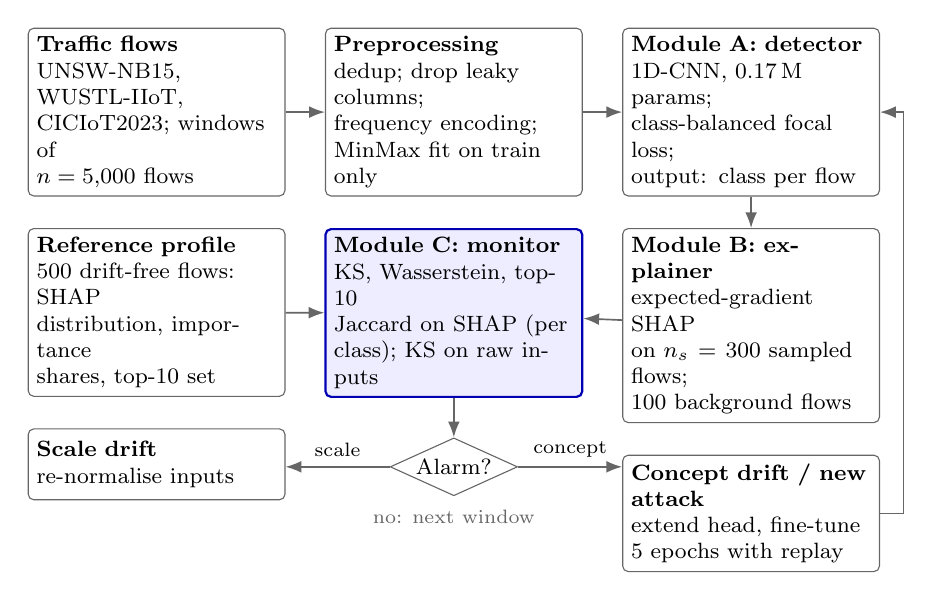
\begin{tikzpicture}[font=\footnotesize, node distance=4mm and 5mm,
  box/.style={draw=black!60, rounded corners=2pt, align=left, inner sep=3pt, text width=3.05cm, minimum height=1.25cm},
  core/.style={box, draw=blue!70!black, fill=blue!7, line width=0.8pt},
  arr/.style={-{Latex[length=2mm]}, draw=black!60, line width=0.6pt}]
\node[box] (data) {\textbf{Traffic flows}\\UNSW-NB15, WUSTL-IIoT,\\CICIoT2023; windows of\\$n=5{,}000$ flows};
\node[box, right=of data] (prep) {\textbf{Preprocessing}\\dedup; drop leaky columns;\\frequency encoding;\\MinMax fit on train only};
\node[box, right=of prep] (A) {\textbf{Module A: detector}\\1D-CNN, 0.17\,M params;\\class-balanced focal loss;\\output: class per flow};
\node[box, below=of A] (B) {\textbf{Module B: explainer}\\expected-gradient SHAP\\on $n_s=300$ sampled flows;\\100 background flows};
\node[core, below=of prep] (C) {\textbf{Module C: monitor}\\KS, Wasserstein, top-10\\Jaccard on SHAP (per\\class); KS on raw inputs};
\node[box, below=of data] (ref) {\textbf{Reference profile}\\500 drift-free flows: SHAP\\distribution, importance\\shares, top-10 set};
\node[draw=black!60, diamond, aspect=2.2, inner sep=1pt, below=5mm of C] (alarm) {Alarm?};
\node[box, below=4mm of ref, minimum height=0.9cm] (scale) {\textbf{Scale drift}\\re-normalise inputs};
\node[box, below=4mm of B, minimum height=0.9cm] (concept) {\textbf{Concept drift / new attack}\\extend head, fine-tune\\5 epochs with replay};
\draw[arr] (data) -- (prep);
\draw[arr] (prep) -- (A);
\draw[arr] (A) -- (B);
\draw[arr] (B) -- (C);
\draw[arr] (ref) -- (C);
\draw[arr] (C) -- (alarm);
\draw[arr] (alarm.west) -- node[above, font=\scriptsize]{scale} (scale.east |- alarm.west);
\draw[arr] (alarm.east) -- node[above, font=\scriptsize]{concept} (concept.west |- alarm.east);
\draw[arr] (concept.east) -- ++(3mm,0) |- (A.east);
\node[below=0.5mm of alarm, font=\scriptsize, text=black!60] {no: next window};
\end{tikzpicture}}
\caption{XDA-IDS architecture. Module A runs on the real-time detection path; Modules B and C monitor sampled flows without labels, and only a concept-drift alarm triggers retraining.}
\label{fig:arch}
\end{figure*}

\subsection{Module A: rare-class-aware detector}
The detector keeps the base paper's architecture for comparability: Conv1D(64, $k{=}3$)--BN--ReLU--MaxPool(2)--Conv1D(128, $k{=}3$)--BN--ReLU--Dropout(0.5)--Dense(64)--ReLU--Dropout(0.5)--Dense($C$). Each flow is treated as a one-channel sequence of length $d$.

\textit{Categorical encoding.} The base paper drops the categorical fields \texttt{proto}, \texttt{service} and \texttt{state}. XDA-IDS replaces each category $v$ of field $j$ by its relative frequency in the training set,
\begin{equation}
\tilde{x}_j = \hat{P}_{\text{train}}(x_j = v),
\end{equation}
with unseen categories mapped to 0. This keeps one input per field, which matters for edge deployment.

\textit{Loss.} Rare classes are handled in the loss rather than by resampling, which avoids synthetic or duplicated samples. With $p_{i}$ the softmax probability of the true class $y_i$ of flow $i$ and $n_c$ the number of training flows in class $c$, the class-balanced focal loss~\cite{lin2017,cui2019} is
\begin{equation}
\mathcal{L}(\theta) = -\frac{1}{N}\sum_{i=1}^{N} \alpha_{y_i}\,(1-p_{i})^{\gamma}\log p_{i},
\end{equation}
\begin{equation}
\alpha_c = C\,\frac{(1-\beta)/(1-\beta^{n_c})}{\sum_{c'=1}^{C}(1-\beta)/(1-\beta^{n_{c'}})},
\end{equation}
where $N$ is the number of flows in a batch, $\gamma=2$ focuses training on hard flows and $\beta=0.9999$ sets the effective-number weighting. The model is trained with Adam and early stopping on validation Macro-F1.

\subsection{Module B: SHAP explainer}
For a flow $\mathbf{x}$ with predicted class $\hat{c}$, the attribution of feature $j$ is computed with expected gradients~\cite{erion2021}, the SHAP approximation implemented by \texttt{GradientExplainer}:
\begin{equation}
\phi_j(\mathbf{x}) = \mathbb{E}_{\mathbf{x}'\sim\mathcal{B},\,\lambda\sim U(0,1)}\!\left[(x_j-x'_j)\,\frac{\partial f_\theta(\mathbf{x}'+\lambda(\mathbf{x}-\mathbf{x}'))_{\hat{c}}}{\partial x_j}\right],
\end{equation}
where $\mathcal{B}$ is a background set of 100 training flows and the expectation is estimated with 50 samples. A \textit{reference profile} is built from $n_r=500$ drift-free validation flows. It stores their attribution matrix $\Phi_{\text{ref}}\in\mathbb{R}^{n_r\times d}$, their predicted classes, the per-feature standard deviation $\sigma_j$ of the attributions, the importance shares $s_j=\overline{|\phi_j|}/\sum_{j'}\overline{|\phi_{j'}|}$ and the top-10 feature set $T_{\text{ref}}$.

\subsection{Module C: SHAP-drift monitor}
For each window $W_t$, the monitor explains a random sample of $n_s=300$ flows, giving $\Phi_t$. It computes four statistics:
\begin{itemize}
\item \textit{SHAP shift count} $K_t$: the number of features whose two-sample KS test between $\Phi_{\text{ref}}$ and $\Phi_t$ is significant at a Bonferroni-corrected level $\alpha/(d\,G)$, over $G$ groups (all flows, and each predicted class with at least 30 flows in both sets), with family-wise $\alpha=0.01$;
\item \textit{effect size} $D_t=\max_j W_1(\Phi_{\text{ref},j},\Phi_{t,j})/\sigma_j$, the largest normalised Wasserstein distance;
\item \textit{reasoning overlap} $J_t=|T_{\text{ref}}\cap T_t|/|T_{\text{ref}}\cup T_t|$, the Jaccard overlap of the top-10 sets;
\item \textit{input shift count} $K^{\text{in}}_t$: the same KS count on raw scaled inputs.
\end{itemize}
The alarm is
\begin{equation}
a_t = [K_t\ge m]\lor[D_t>\omega]\lor[J_t<\tau]\lor[K^{\text{in}}_t\ge m_{\text{in}}].
\end{equation}
The thresholds $m$, $\omega$, $\tau$ and $m_{\text{in}}$ are set on 20 drift-free calibration windows, disjoint from the reference profile, as quantiles that split a target false-alarm rate (FAR) of 0.05 across the SHAP signals. Because raw attributions move whenever inputs move, the diagnosis compares importance shares rather than raw values: an alarm is diagnosed as concept drift if $\|\mathbf{s}_t-\mathbf{s}_{\text{ref}}\|_1$ exceeds its calibrated threshold or $J_t<\tau$, and as scale drift otherwise. The alarm reports $\mathcal{S}_t$, the five features with the largest normalised Wasserstein distance. Algorithm~\ref{alg:monitor} summarises the procedure.

\begin{algorithm}[t]
\caption{SHAP-drift monitoring of one window}
\label{alg:monitor}
\small
\begin{algorithmic}[1]
\Require window $W_t$; detector $f_\theta$; explainer; reference profile $(\Phi_{\text{ref}},T_{\text{ref}},\mathbf{s}_{\text{ref}},\boldsymbol\sigma)$; thresholds $m,\omega,\tau,m_{\text{in}},\rho$
\Ensure alarm $a_t$, shifted features $\mathcal{S}_t$, diagnosis $\delta_t$
\State $X_t \gets$ random sample of $n_s$ flows from $W_t$
\State $\hat{\mathbf{y}}_t \gets \arg\max f_\theta(X_t)$; \quad $\Phi_t \gets$ SHAP$(X_t,\hat{\mathbf{y}}_t)$
\State $K_t \gets$ \# features with KS $p<\alpha/(dG)$ on $\Phi$ (overall and per class)
\State $K^{\text{in}}_t \gets$ the same count on $X_t$
\State $D_t \gets \max_j W_1(\Phi_{\text{ref},j},\Phi_{t,j})/\sigma_j$; \quad $J_t \gets \text{Jaccard}(T_{\text{ref}},T_t)$
\State $a_t \gets [K_t\ge m]\lor[D_t>\omega]\lor[J_t<\tau]\lor[K^{\text{in}}_t\ge m_{\text{in}}]$
\If{not $a_t$} \State $\delta_t\gets$ \textit{none}
\ElsIf{$\|\mathbf{s}_t-\mathbf{s}_{\text{ref}}\|_1>\rho$ \textbf{or} $J_t<\tau$} \State $\delta_t\gets$ \textit{concept} \Comment{retrain}
\Else \State $\delta_t\gets$ \textit{scale} \Comment{re-normalise}
\EndIf
\State $\mathcal{S}_t\gets$ top-5 features by $W_1/\sigma_j$
\State \Return $(a_t,\mathcal{S}_t,\delta_t)$
\end{algorithmic}
\end{algorithm}

\subsection{Retraining loop}
After a concept-drift alarm, an analyst labels the alarmed window. If it contains a new attack family, the output layer is extended by one unit per new class while existing weights are kept. The detector is then fine-tuned for 5 epochs at learning rate $10^{-4}$ on the labelled window mixed with an equal-sized replay sample of the original training data, and the reference profile is rebuilt.

\subsection{Changes after the Phase 2 feedback}
Feedback on the methodology asked for a fuller set of evaluation metrics. The base paper reports only accuracy, precision, recall and F1; XDA-IDS is evaluated with Macro-F1, per-class recall, FPR, Matthews correlation coefficient (MCC), PR-AUC, drift-detection delay and false-alarm rate, diagnosis and localisation accuracy, explanation fidelity and stability, and latency and memory (Section~\ref{sec:setup}). Three further changes arose during implementation. The diagnosis rule compares importance shares instead of raw SHAP values, for the reason given above. A leakage audit was added (Section~\ref{sec:setup}-B). The online-learning baseline uses a sliding-window KNN because the installed River library~\cite{montiel2021} has no SAM-KNN.

% ============================================================== SETUP
\section{Experimental Setup}\label{sec:setup}
\subsection{Datasets}
Table~\ref{tab:data} lists the datasets, all obtained from public Kaggle mirrors. UNSW-NB15 and WUSTL-IIoT-2021~\cite{zolanvari2021} are the base paper's datasets; CICIoT2023~\cite{neto2023} adds recent IoT traffic for transfer experiments. Class imbalance is severe: Worms are 0.07\% of the larger UNSW-NB15 partition, and Backdoor and Command Injection are about 0.02\% each of WUSTL-IIoT-2021.

\begin{table}[t]
\caption{Datasets used}
\label{tab:data}
\centering\footnotesize
\begin{tabular}{@{}lrcl@{}}
\toprule
Dataset & Raw flows & Classes & Use \\
\midrule
UNSW-NB15 (both partitions) & 257{,}673 & 10 & E1--E4 \\
WUSTL-IIoT-2021 & 1{,}194{,}464 & 5 & E1, E2, E4 \\
CICIoT2023 (1\,M sample) & 1{,}000{,}000 & 8 & E5 \\
\bottomrule
\end{tabular}
\end{table}

\subsection{Preprocessing and leakage audit}
Before training, a data audit checked each dataset for label leakage. It found three problems in the protocol used by the base paper: (i) the UNSW-NB15 \texttt{id} column, a row index, correlates with the label ($r=-0.39$ and $+0.73$ in the two partitions) because rows are ordered by class; (ii) the WUSTL-IIoT-2021 \texttt{Target} column equals the binary label on 100\% of rows; and (iii) 32.0\% and 38.6\% of UNSW-NB15 rows are exact duplicates. The XDA protocol therefore removes infinite and missing values and duplicate rows, drops \texttt{id}, \texttt{Target}, timestamps, IP addresses and ports, frequency-encodes categorical fields, and fits MinMax scaling on the training split only. Outlier removal is not applied, because attacks are often outliers. To quantify the leakage, the base paper's protocol is also reproduced exactly (\textit{base\_repro}: index and label columns kept, categorical fields dropped, scaler fitted on all rows, no deduplication).

After deduplication, UNSW-NB15 has 102{,}528 training and 48{,}824 test flows (42 features) and WUSTL-IIoT-2021 has 730{,}522 training and 347{,}868 test flows (39 features).

\subsection{Data splits and experiments}
\textit{Split A} (static) is a stratified 70/30 train/test split with 10\% of the training part held out for early stopping. Six experiments are run:
\begin{itemize}
\item \textbf{E1/E2} static detection and rare-class analysis on Split A;
\item \textbf{E3} unseen attack families: one family (Exploits, DoS or Backdoor) is removed from training; a stream of 20 windows of 5{,}000 flows is built, and from window 10 the held-out family forms 20\% of each window;
\item \textbf{E4} injected drift: byte and packet volume features are scaled by $3\times$ from window 10 in four patterns (sudden; gradual, where the share of scaled flows rises over 5 windows; incremental, where the factor rises from 1 to 3; recurring, where drifted and clean blocks alternate), plus a class-mixture stream in which DoS forms 50\% of each window, plus WUSTL-IIoT-2021 replayed in time order;
\item \textbf{E5} cross-dataset transfer between UNSW-NB15 and CICIoT2023 on seven harmonised features (duration, rate, TTL, mean packet size, total bytes, protocol, service), binary task;
\item \textbf{E6} detector and monitor cost.
\end{itemize}

\subsection{Baselines}
Detector baselines are the base paper's CNN in two forms (\textit{base\_repro} and the leak-free \textit{base\_clean}), an LSTM(64) as in the base paper, Random Forest (100 trees)~\cite{pedregosa2011}, XGBoost (300 trees, depth 8)~\cite{chen2016xgb} and the RF + Isolation Forest hybrid of Obaidat \textit{et al.}~\cite{obaidat2026}. Monitor baselines are KS on inputs~\cite{obaidat2026}, KS on prediction confidence, KSWIN~\cite{raab2020}, and the label-based ADWIN~\cite{bifet2007} and DDM~\cite{gama2004} on the error stream.

\subsection{Evaluation metrics}
Detection is measured by accuracy, Macro-F1 (primary, because of class imbalance), weighted F1, macro precision and recall, MCC, FPR (share of normal flows flagged), detection rate (share of attack flows flagged as any attack), PR-AUC and per-class recall. Monitors are measured by the number of scenarios detected, detection delay in windows after onset and FAR on pre-onset windows. Explanations are measured by fidelity (Macro-F1 drop when the top-$k$ SHAP features are zeroed, against $k$ random features), stability (top-10 Jaccard over 20 bootstraps) and localisation (share of reported shifted features that were actually perturbed). Efficiency is measured by latency per flow on one CPU thread, throughput, parameters and model size.

\subsection{Implementation and reproducibility}
XDA-IDS is implemented in Python 3.11.9 with PyTorch 2.11.0 (CUDA 12.8)~\cite{paszke2019}, scikit-learn 1.9.1, XGBoost 3.2.0, SHAP 0.51.0, River 0.27.0 and pandas 2.3.3. Experiments ran on an AMD Ryzen 5 3600 CPU (6 cores), 16\,GB RAM and an NVIDIA GTX 1660 Ti GPU (6\,GB) under Windows 11. Table~\ref{tab:hyper} lists the hyperparameters. All reported results use random seed 1, a maximum of 10 epochs with patience 10 and batch size 512; the complete pipeline ran in 2.71 hours. Code, configuration, per-run results and logs are public~\cite{repo}; \texttt{python run\_all.py -{}-quick} reproduces every number in this paper.

\begin{table}[t]
\caption{Hyperparameters}
\label{tab:hyper}
\centering\footnotesize
\begin{tabular}{@{}ll@{}}
\toprule
Parameter & Value \\
\midrule
Optimiser; batch size; learning rate & Adam; 512; $2\times10^{-3}$ \\
Max epochs; early-stopping patience & 10; 10 (validation Macro-F1) \\
CNN filters; kernel; dense units; dropout & 64/128; 3; 64; 0.5 \\
Focal loss $\gamma$; $\beta$ & 2.0; 0.9999 \\
SHAP background; reference; sample $n_s$ & 100; 500; 300 flows \\
Window $n$; family-wise $\alpha$; target FAR & 5{,}000; 0.01; 0.05 \\
Fine-tuning epochs; learning rate & 5; $10^{-4}$ \\
RF trees; XGBoost trees, depth, rate & 100; 300, 8, 0.1 \\
Isolation Forest contamination & 0.01 \\
\bottomrule
\end{tabular}
\end{table}

% ============================================================== RESULTS
\section{Results and Analysis}\label{sec:results}
\subsection{Static detection (E1)}
Table~\ref{tab:detect} reports multiclass results. On UNSW-NB15, XGBoost is the most accurate detector (Macro-F1 0.584). XDA-IDS has the highest detection rate of all models (0.980) and the highest macro recall among the CNN-based models (0.554), but the lowest accuracy (0.668) and the highest FPR (0.264). On WUSTL-IIoT-2021 every model exceeds 0.99 accuracy; Macro-F1 differences come from the 64 Backdoor and 77 Command Injection test flows. On the binary tasks, XDA-IDS reaches Macro-F1 0.897 on UNSW-NB15 (\textit{base\_clean}: 0.899) and 0.999 on WUSTL-IIoT-2021. XDA-IDS processes a flow in 0.24\,ms, 12$\times$ faster than XGBoost and 31$\times$ faster than Random Forest, with a 0.67\,MB model.

\begin{table}[t]
\caption{Multiclass detection results on Split A (seed 1). Best value per column in bold.}
\label{tab:detect}
\centering\footnotesize
\begin{tabular}{@{}lcccccc@{}}
\toprule
Model & Acc & Macro-F1 & Macro-R & FPR & DR & ms/flow \\
\midrule
\multicolumn{7}{@{}l}{\textit{UNSW-NB15 (10 classes, 48{,}824 test flows)}} \\
base\_clean CNN & 0.744 & 0.356 & 0.384 & 0.145 & 0.916 & 0.224 \\
LSTM & 0.732 & 0.348 & 0.348 & 0.079 & 0.794 & \textbf{0.176} \\
Random Forest & 0.817 & 0.544 & 0.524 & 0.060 & 0.900 & 7.290 \\
RF + IF~\cite{obaidat2026} & 0.813 & 0.543 & 0.524 & 0.069 & 0.901 & 14.996 \\
XGBoost & \textbf{0.823} & \textbf{0.584} & 0.575 & \textbf{0.052} & 0.896 & 2.876 \\
XDA-IDS & 0.668 & 0.409 & \textbf{0.554}$^\dagger$ & 0.264 & \textbf{0.980} & 0.235 \\
\midrule
\multicolumn{7}{@{}l}{\textit{WUSTL-IIoT-2021 (5 classes, 347{,}868 test flows)}} \\
base\_clean CNN & \textbf{1.000} & 0.947 & 0.923 & \textbf{0.000} & 0.998 & 0.222 \\
LSTM & 0.999 & 0.920 & 0.875 & \textbf{0.000} & 0.993 & \textbf{0.180} \\
Random Forest & \textbf{1.000} & 0.964 & 0.948 & \textbf{0.000} & 0.999 & 7.186 \\
RF + IF~\cite{obaidat2026} & 0.991 & 0.799 & 0.946 & 0.010 & 0.999 & 14.788 \\
XGBoost & \textbf{1.000} & \textbf{0.980} & \textbf{0.965} & \textbf{0.000} & 0.999 & 0.383 \\
XDA-IDS & 0.999 & 0.940 & 0.920 & \textbf{0.000} & 0.985 & 0.236 \\
\bottomrule
\multicolumn{7}{@{}l}{\scriptsize Macro-R: macro recall; DR: detection rate. $^\dagger$Highest among CNN-based models;}\\
\multicolumn{7}{@{}l}{\scriptsize XGBoost's 0.575 is higher overall.}
\end{tabular}
\end{table}

\subsection{Rare-class detection (E2)}
Fig.~\ref{fig:recall} shows per-class recall on UNSW-NB15. Four classes that the leak-free base CNN never detects gain recall with XDA-IDS: Worms (0.88), Analysis (0.81), Shellcode (0.45) and Backdoor (0.08). The base paper's own confusion matrix also shows zero recall for Backdoor, Shellcode and Worms. The cost falls on Normal ($-0.12$), Exploits ($-0.19$) and Reconnaissance ($-0.50$). Fig.~\ref{fig:confusion} shows why: the base CNN collapses rare classes into Exploits and Reconnaissance (75\% of Worms become Exploits), whereas XDA-IDS separates them but sends 23\% of Normal flows to Fuzzers and 73\% of Backdoor flows to Analysis. Focal loss thus moves errors from \textit{rare class missed} to \textit{rare classes confused with each other} and \textit{normal traffic flagged}.

\begin{figure}[t]
\centering
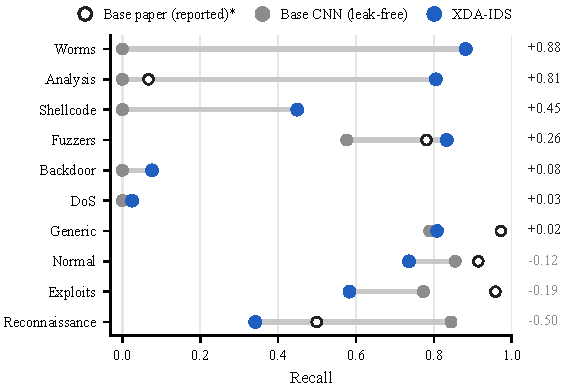
\includegraphics[width=\columnwidth]{figures/fig_recall.pdf}
\caption{Per-class recall on UNSW-NB15 multiclass, sorted by the change from the leak-free base CNN (right column). $^{*}$Values read from the base paper's confusion matrix~\cite{udurume2026}.}
\label{fig:recall}
\end{figure}

\begin{figure*}[t]
\centering
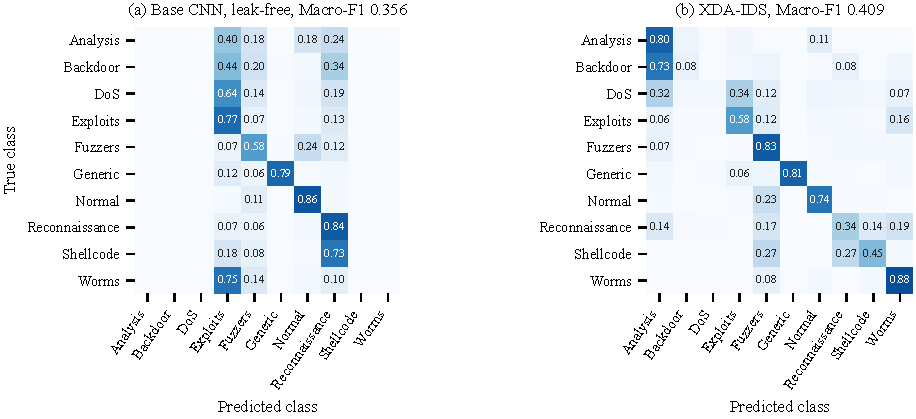
\includegraphics[width=0.92\textwidth]{figures/fig_confusion.pdf}
\caption{Row-normalised confusion matrices on UNSW-NB15 multiclass (values $\ge0.05$ shown). (a) The leak-free base CNN maps rare classes to Exploits and Reconnaissance. (b) XDA-IDS recovers Analysis and Worms but confuses Backdoor with Analysis and Normal with Fuzzers.}
\label{fig:confusion}
\end{figure*}

\subsection{Drift and unseen-attack detection (E3, E4)}
Table~\ref{tab:monitor} and Fig.~\ref{fig:monitors} compare the monitors over the 11 scenarios with a known onset. All three SHAP-based monitors detect every scenario. Input KS misses the unseen DoS family, because DoS flows resemble known traffic in raw features; SHAP KS detects it once the model's reasoning changes. KSWIN also detects all scenarios but with a 0.209 FAR. The label-based ADWIN and DDM detect only 6 and 4 scenarios. Fig.~\ref{fig:timeline} shows the unseen-DoS stream window by window. The full XDA monitor raises 2 false alarms before onset there, which illustrates its main weakness: a FAR of 0.164 against the 0.05 target. Its KS-only variant meets the target (0.009).

\begin{table}[t]
\caption{Drift monitors over 11 scenarios with known onset (E3, E4)}
\label{tab:monitor}
\centering\footnotesize
\begin{tabular}{@{}lcccc@{}}
\toprule
Monitor & Labels & Detected & Delay (win.) & FAR \\
\midrule
XDA (SHAP + input KS) & no & \textbf{11/11} & 0.27 & 0.164 \\
SHAP signals only & no & \textbf{11/11} & 0.36 & 0.118 \\
SHAP KS only & no & \textbf{11/11} & 0.55 & 0.009 \\
Input KS~\cite{obaidat2026} & no & 10/11 & \textbf{0.10} & \textbf{0.000} \\
Confidence KS & no & 7/11 & 0.71 & 0.009 \\
KSWIN~\cite{raab2020} & no & \textbf{11/11} & 1.00 & 0.209 \\
ADWIN~\cite{bifet2007} & yes & 6/11 & 4.50 & \textbf{0.000} \\
DDM~\cite{gama2004} & yes & 4/11 & 0.00 & 0.327 \\
\bottomrule
\end{tabular}
\end{table}

\begin{figure}[t]
\centering
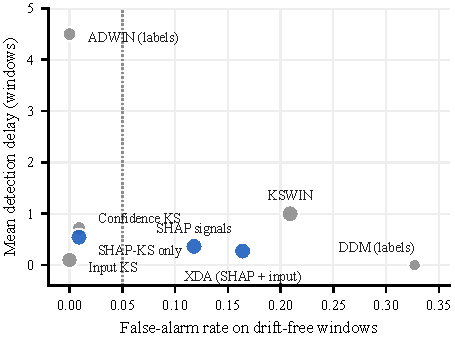
\includegraphics[width=\columnwidth]{figures/fig_monitors.pdf}
\caption{Detection delay against false-alarm rate for each monitor over 11 scenarios (lower left is better; marker size grows with the number of scenarios detected). Blue: SHAP-based monitors. Dotted line: the 0.05 target FAR.}
\label{fig:monitors}
\end{figure}

\begin{figure}[t]
\centering
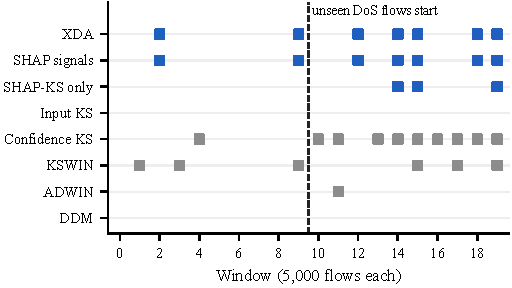
\includegraphics[width=\columnwidth]{figures/fig_timeline.pdf}
\caption{Alarms per window in the unseen-DoS stream on UNSW-NB15 (E3). Input KS never fires; the SHAP monitors fire after onset, and the full XDA monitor also fires twice before it.}
\label{fig:timeline}
\end{figure}

\subsection{Diagnosis and localisation}
Table~\ref{tab:diag} reports, for the XDA monitor, how often its diagnosis is correct and how many of its reported shifted features were actually perturbed. Unseen attack families are diagnosed as concept drift in 80--100\% of windows, and 60--86\% of the reported features are the ones that were scaled. However, scale drift is diagnosed correctly in only 0--30\% of windows: scaling the volume features also changes their share of the model's attributions, which the rule reads as a change in reasoning. On the WUSTL-IIoT-2021 stream in natural time order, every SHAP and input monitor alarms in all windows, led by the TTL feature \texttt{dTtl}; this stream drifts continuously and needs a refreshed reference profile.

\begin{table}[t]
\caption{XDA monitor diagnosis and localisation per scenario}
\label{tab:diag}
\centering\footnotesize
\begin{tabular}{@{}llccc@{}}
\toprule
Dataset & Scenario & Delay & Diagnosis correct & Localised \\
\midrule
UNSW & unseen DoS & 2 & 80\% & -- \\
UNSW & unseen Exploits & 0 & 100\% & -- \\
UNSW & class mixture (DoS) & 0 & 100\% & -- \\
UNSW & sudden / gradual & 0 / 1 & 0\% / 0\% & 86\% / 84\% \\
UNSW & incremental / recurring & 0 / 0 & 10\% / 0\% & 82\% / 73\% \\
WUSTL & sudden / gradual & 0 / 0 & 0\% / 30\% & 66\% / 66\% \\
WUSTL & incremental / recurring & 0 / 0 & 10\% / 0\% & 62\% / 60\% \\
\bottomrule
\end{tabular}
\end{table}

\subsection{Explanation quality}
Masking the top-1, 3 and 5 SHAP features lowers UNSW-NB15 Macro-F1 by 0.122, 0.242 and 0.255, against 0.018, 0.010 and 0.042 for the same number of random features; on WUSTL-IIoT-2021 the drops are 0.611, 0.661 and 0.742 against 0.171, 0.294 and 0.388. The explanations are therefore faithful. The top-10 set is identical across 20 bootstraps on UNSW-NB15 (Jaccard 1.00) and nearly so on WUSTL-IIoT-2021 (mean 0.98, minimum 0.82). The top-ranked features are TTL values on both datasets (\texttt{sttl}, \texttt{dttl} on UNSW-NB15; \texttt{dTtl}, \texttt{sTtl} on WUSTL-IIoT-2021), which reflect how each testbed was built rather than attack behaviour.

\subsection{Cross-dataset transfer (E5)}
A binary model trained on UNSW-NB15 reaches in-domain Macro-F1 0.826 but 0.455 on CICIoT2023, with an FPR of 0.992; the reverse direction falls from 0.700 to 0.281 (FPR 0.998). Neither direction transfers. The monitor alarms on 100\% of cross-domain windows and diagnoses concept drift, led by \texttt{duration}, \texttt{mean\_pkt} and \texttt{proto}, so it would flag a model deployed on the wrong network.

\subsection{Edge cost (E6) and retraining}
On one CPU thread the detector has a latency of 0.235\,ms per flow and a batched throughput of 27{,}173 flows per second, with 173.5\,K parameters. Computing SHAP for a 300-flow sample takes 9.4--12.0\,s per window on the GPU and the monitor statistics 0.29--0.64\,s with under 0.5\,MB of memory; this runs off the detection path. After an unseen-family alarm, the retraining loop adapted the detector at window 10 (Exploits, Backdoor) or 18 (DoS), and post-adaptation binary detection accuracy was 0.857--0.881, at or above the pre-onset level (0.834--0.865).

\subsection{Statistical evidence}
Because all results come from one seed, uncertainty is estimated on the test set. Bootstrap 95\% confidence intervals of UNSW-NB15 multiclass Macro-F1 do not overlap: [0.404, 0.415] for XDA-IDS and [0.354, 0.359] for \textit{base\_clean}. McNemar's test on per-flow predictions is significant in both directions of the trade-off: on UNSW-NB15 multiclass, \textit{base\_clean} is correct where XDA-IDS is wrong on 6{,}534 flows and the reverse holds on 2{,}855 ($p<0.001$), reflecting the higher accuracy of \textit{base\_clean} on majority classes; on the binary task the split is 967 to 879 ($p=0.043$).

% ============================================================== BASE PAPERS
\section{Comparison with Base Papers and State of the Art}\label{sec:base}
\subsection{Base papers}
XDA-IDS builds on two base papers (Table~\ref{tab:base}): Udurume \textit{et al.}~\cite{udurume2026}, whose explainable 1D-CNN is the detector XDA-IDS extends, and Obaidat \textit{et al.}~\cite{obaidat2026}, whose hybrid RF + Isolation Forest + input-KS system is the closest drift-aware IDS and is re-implemented here as a baseline.

\begin{table*}[t]
\caption{Summary of the base papers (results as reported by their authors)}
\label{tab:base}
\centering\footnotesize
\begin{tabular}{@{}L{2.3cm}L{2.4cm}L{2.7cm}L{2.0cm}L{2.0cm}L{2.5cm}L{2.9cm}@{}}
\toprule
Base paper & Problem & Method & Dataset & Metrics & Reported results & Key limitations \\
\midrule
Udurume, Shakhov \& Koo, 2026~\cite{udurume2026} & Lightweight, explainable IoT/IIoT IDS & 1D-CNN vs LSTM; SHAP DeepExplainer; fidelity and stability tests; top-$k$ pruning & UNSW-NB15, WUSTL-IIoT-2021 & Acc, P, R, F1; time, memory & F1 97.5\% / 94.0\% (UNSW bin./multi); 2.18\,ms; 22.1\,MB & Static split; label leakage; rare classes at 0 recall; 8.4\% FPR; SHAP offline only \\
Obaidat, Abouali \& Shakeel, 2026~\cite{obaidat2026} & Drift-aware IoT IDS & RF + benign-only Isolation Forest + KS on inputs; one held-out family & CICIoT2023 (3.89\,M flows) & Acc, P, R, F1, FPR, balanced acc. & Acc 99.73\%, FPR 4.77\%; 85.26\% detection of held-out family & Binary only; one dataset; hybrid below RF alone; input-only drift signal; no XAI \\
\bottomrule
\end{tabular}
\end{table*}

\subsection{Quantitative comparison}
Table~\ref{tab:quant} places XDA-IDS beside the base paper on UNSW-NB15. Values marked $^{*}$ are taken from the original paper. Values marked $^{\ddagger}$ come from running the base paper's published notebooks unchanged, apart from loading data from Kaggle. All other values were produced in this work: \textit{base\_repro} re-implements the base protocol, and \textit{base\_clean} applies the leak-free protocol to the same CNN.

\begin{table}[t]
\caption{Comparison with the base paper~\cite{udurume2026} on UNSW-NB15}
\label{tab:quant}
\centering\footnotesize
\begin{tabular}{@{}lccccc@{}}
\toprule
& \multicolumn{2}{c}{Binary} & \multicolumn{2}{c}{Multiclass} & \\
\cmidrule(lr){2-3}\cmidrule(lr){4-5}
Source & Acc & FPR & Acc & Macro-F1 & ms/flow \\
\midrule
Base paper, reported & 0.975\paperval & 0.084\paperval & 0.941\paperval & 0.940\paperval$^{\S}$ & 2.18\paperval \\
Base paper, its code & 0.968$^{\ddagger}$ & -- & 0.810$^{\ddagger}$ & 0.41$^{\ddagger}$ & -- \\
base\_repro (leaky) & 0.986 & 0.026 & 0.857 & 0.433 & 0.240 \\
base\_clean (leak-free) & 0.899 & 0.100 & 0.744 & 0.356 & 0.224 \\
\textbf{XDA-IDS} & 0.897 & 0.119 & 0.668 & 0.409 & 0.235 \\
\bottomrule
\multicolumn{6}{@{}l}{\scriptsize $^{*}$From~\cite{udurume2026}. $^{\ddagger}$Base paper's notebooks run by us. $^{\S}$Averaging not stated.}
\end{tabular}
\end{table}

\subsection{Methodological comparison}
XDA-IDS differs from Udurume \textit{et al.} in four ways, each aimed at one of its limitations: (i) a leak-free protocol replaces a split in which the label is partly encoded in the inputs; (ii) a class-balanced focal loss replaces cross-entropy, addressing zero rare-class recall; (iii) categorical fields are encoded rather than dropped; and (iv) SHAP becomes an online monitoring signal instead of an offline report. Compared with Obaidat \textit{et al.}, XDA-IDS monitors the model's attributions rather than only its inputs, which allows it to detect attacks that look normal in raw features and to name the features whose role changed; it also handles multiclass detection and is evaluated on three datasets and three held-out families instead of one.

\subsection{Improvement analysis}
Against the re-implemented leak-free base CNN on UNSW-NB15 multiclass, XDA-IDS improves Macro-F1 by $+0.053$ (+14.9\% relative), macro recall by $+0.170$ (+44.3\%) and detection rate by $+0.064$ (+7.0\%). The gain comes from the focal loss (Section~\ref{sec:ablation}): it is concentrated in four rare classes, whose recall rises by 0.08--0.88. Against the base paper's reported figures, XDA-IDS has 89\% lower latency per flow (0.235 vs 2.18\,ms$^{*}$) with 83\% fewer parameters (0.17\,M vs 1.02\,M$^{*}$), and its explanations are more faithful (top-3 masking drop 0.242 vs 0.086$^{*}$). Against Obaidat \textit{et al.}'s input-KS signal, the SHAP-KS monitor detects one more scenario (11 vs 10 of 11, +10\%), the unseen DoS family.

XDA-IDS does not outperform the base papers on every metric. Its UNSW-NB15 binary accuracy (0.897) is 7.8 points below the reported 0.975$^{*}$, its multiclass accuracy is 7.6 points below \textit{base\_clean}, its FPR rises by 0.119 over \textit{base\_clean}, and the re-implemented RF + IF hybrid has a higher multiclass Macro-F1 (0.543). The input-KS monitor also responds faster (0.10 vs 0.55 windows) when it does detect a drift.

\subsection{Fairness and limitations of the comparison}
Several factors affect this comparison. (i) The base paper's reported accuracy relies on the leaky protocol: the leaky reproduction reaches 0.986 binary accuracy, so most of the gap to 0.975$^{*}$ is protocol, not model. (ii) Its own notebooks print 0.81 multiclass accuracy and 0.41 Macro-F1 (5 epochs, one seed), so its reported 0.941 could not be reproduced. (iii) The base paper does not state whether its F1 is macro- or weighted-averaged. (iv) In the Kaggle mirror used here the UNSW-NB15 partition files are swapped, so \textit{base\_repro} trained on 82{,}332 rows rather than 175{,}341. (v) This work uses batch size 512 and at most 10 epochs, against 128 and early stopping in the base paper. (vi) Latency was measured on different, partly unstated hardware. (vii) Obaidat \textit{et al.} report binary results on CICIoT2023, so only their method, not their numbers, is compared directly.

\subsection{Position among recent studies}
Among the studies in Table~\ref{tab:related}, only Sharma \textit{et al.}~\cite{sharma2025} (accuracy 97.9\%$^{*}$) and Nasir \textit{et al.}~\cite{nasir2026} (92.1\%$^{*}$) report UNSW-NB15 results, and neither checks for leakage. XDA-IDS has lower per-flow latency (0.24\,ms) than the base paper (2.18\,ms$^{*}$), Aly and Alotaibi (10.2\,ms$^{*}$) and Nasir \textit{et al.} (18--22\,ms$^{*}$); Sharma \textit{et al.} report under 3\,ms$^{*}$ on a cloud GPU. It is also the only study that validates its explanations, uses them for label-free monitoring and tests unseen families, injected drift and cross-dataset transfer together.

% ============================================================== ABLATION
\section{Ablation Study}\label{sec:ablation}
\subsection{Detector components}
Table~\ref{tab:ablation} changes one component at a time. Removing leakage costs 0.086 binary Macro-F1 on UNSW-NB15 (0.985 to 0.899), showing that most of the base protocol's advantage is leakage. Focal loss is the component that recovers rare classes: it adds $+0.053$ multiclass Macro-F1 over \textit{base\_clean} and is the only change that lifts Worms and Analysis recall above zero. Frequency encoding alone adds $+0.029$ Macro-F1 and halves FPR (0.145 to 0.073), but adds nothing on top of focal loss and, combined with it, triples FPR (0.087 to 0.264). Local SHAP explanations of errors point to the encoded \texttt{proto} field, which DoS, Analysis and Backdoor share. On binary tasks and on WUSTL-IIoT-2021 all variants lie within 0.014 Macro-F1; WUSTL-IIoT-2021 has no categorical fields left after identifiers are dropped.

\begin{table}[t]
\caption{Detector ablation (Macro-F1 unless stated). LF: leak-free; FE: frequency encoding; FL: focal loss.}
\label{tab:ablation}
\centering\footnotesize
\begin{tabular}{@{}lccccccc@{}}
\toprule
Variant & LF & FE & FL & \shortstack{UNSW\\bin.} & \shortstack{UNSW\\multi} & \shortstack{UNSW\\FPR} & \shortstack{WUSTL\\multi} \\
\midrule
base\_repro & -- & -- & -- & 0.985 & 0.433 & 0.021 & 0.934 \\
base\_clean & \checkmark & -- & -- & 0.899 & 0.356 & 0.145 & \textbf{0.947} \\
no focal loss & \checkmark & \checkmark & -- & \textbf{0.901} & 0.385 & \textbf{0.073} & 0.942 \\
no encoding & \checkmark & -- & \checkmark & 0.887 & \textbf{0.409} & 0.087 & 0.943 \\
XDA-IDS (full) & \checkmark & \checkmark & \checkmark & 0.897 & \textbf{0.409} & 0.264 & 0.940 \\
\bottomrule
\end{tabular}
\end{table}

\subsection{Monitor components}
Table~\ref{tab:monitor} doubles as the monitor ablation. Removing the Wasserstein and Jaccard signals (SHAP KS only) keeps 11/11 detections and lowers FAR from 0.118 to 0.009 at about 0.2 windows more delay, so those two signals add false alarms rather than detections in this setting. Adding input KS to the SHAP signals (full XDA) shortens the delay from 0.36 to 0.27 windows but raises FAR to 0.164. Removing SHAP entirely (input KS only) loses the unseen DoS family.

\subsection{Feature subset}
Fig.~\ref{fig:topk} retrains the detector on the top-$k$ SHAP features. On UNSW-NB15 the top 15 features reach Macro-F1 0.429, above all 42 features (0.422), with 58.8\,K parameters instead of 173.5\,K and twice the throughput. On WUSTL-IIoT-2021 the top 5 features (0.931) exceed all 39 (0.917).

\begin{figure}[t]
\centering
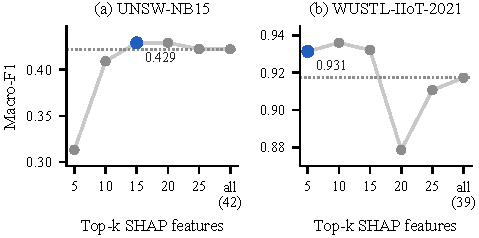
\includegraphics[width=\columnwidth]{figures/fig_topk.pdf}
\caption{Macro-F1 of the detector retrained on the top-$k$ SHAP features. Dotted line: all features. Blue: smallest $k$ that matches or exceeds it.}
\label{fig:topk}
\end{figure}

% ============================================================== DISCUSSION
\section{Discussion}\label{sec:discussion}
\subsection{Why the method works}
A drift monitor on raw inputs sees only whether the data changed. A monitor on attributions sees whether the model now relies on different evidence. An unseen attack family that resembles known traffic in raw features, such as DoS on UNSW-NB15, still changes which features drive the model's decisions; this is why SHAP KS detected the unseen DoS family while input KS did not. Focal loss works because the class-balanced weights raise the gradient contribution of classes with a few hundred flows, which plain cross-entropy lets the majority classes outweigh.

\subsection{Practical implications}
The detector is small enough for an IoT gateway (0.67\,MB, about 27{,}000 flows per second in batches on one CPU thread). The monitor needs no labels and names the shifted features, so an analyst receives an alarm with a starting point for investigation. At about 10\,s of SHAP computation per window, a fog node can check every window up to roughly 500 flows per second, or a sample of windows at higher rates. SHAP KS only is the better default monitor in this evaluation, given its 0.009 FAR.

\subsection{Limitations and failure cases}
(i) XDA-IDS raises FPR on UNSW-NB15 multiclass to 0.264 and stays below XGBoost in Macro-F1. (ii) The diagnosis rule mislabels scale drift as concept drift in 70--100\% of windows. (iii) The full monitor's FAR (0.164) exceeds its 0.05 target; 12 of its 18 pre-onset alarms were within sampling noise of a threshold, which points to calibration on only 20 windows, where a 0.983 quantile is close to the maximum. (iv) Transfer to CICIoT2023 fails in both directions. (v) WUSTL-IIoT-2021 in natural time order drifts in every window, so a static reference profile is unusable there. (vi) The monitor's SHAP step costs about 10\,s per window.

\subsection{Threats to validity}
\textit{Internal validity:} all results use one seed and at most 10 epochs, so seed-to-seed variance is unknown and some differences (for example, 0.409 against 0.385) may not hold; bootstrap intervals cover test-set sampling only. \textit{Construct validity:} drift is injected synthetically by scaling volume features, which may not match real drift; the diagnosis ground truth assumes scaling is pure scale drift. \textit{External validity:} the top-ranked features on both datasets are TTL values, a known testbed artefact, so accuracy may not carry over to real networks, as the failed transfer suggests. All datasets are lab captures. \textit{Conclusion validity:} the comparison with reported results is affected by the differences listed in Section~\ref{sec:base}-F.

\subsection{Were the objectives met?}
The Phase 2 objective was to make an explainable lightweight IDS drift-aware through its own explanations, while improving rare-attack detection and preserving real-time performance. Of the four research questions, RQ2 (label-free detection of drift and unseen families) is answered positively: 11 of 11 scenarios were detected. RQ1 (rare classes and false positives) is partly met: rare-class recall improves, but FPR rises. RQ3 (localisation and drift-type diagnosis) is partly met: localisation reaches 60--86\%, but scale drift is misdiagnosed. RQ4 (cost) is answered for a desktop CPU and GPU, not for edge hardware. The research gap, using explanations as an operational label-free signal, is therefore closed for the datasets studied, while the false-positive and diagnosis problems remain open.

% ============================================================== CONCLUSION
\section{Conclusion and Future Work}\label{sec:conclusion}
This paper presented XDA-IDS, a lightweight 1D-CNN IDS for IoT/IIoT networks that uses its own SHAP attributions as a label-free drift signal. Under a leak-free protocol, it raised UNSW-NB15 multiclass Macro-F1 over the base CNN from 0.356 to 0.409, recovered three rare attack classes from zero recall, detected all 11 drift and unseen-family scenarios without labels, and classified flows in 0.24\,ms, at the cost of a higher false-positive rate. A leakage audit also showed that the base paper's reported accuracy depends on an index column, a label column and duplicate rows. Future work will repeat the evaluation over five seeds, calibrate the monitor on more windows and adopt SHAP KS as the default signal, base the diagnosis on the perturbed features' importance shares only, test models without TTL features, refresh the reference profile on naturally drifting streams, and measure the system on edge hardware such as a Raspberry Pi.

% ============================================================== DECLARATIONS
\section*{Declarations}
\textit{Data and code availability.} UNSW-NB15, WUSTL-IIoT-2021 and CICIoT2023 are publicly available on Kaggle (mirrors \texttt{mrwellsdavid/unsw-nb15}, \texttt{annaamalaiu/wustl-iiot-2021-dataset} and \texttt{ioannispan/ciciot2023-1m}). Code, configuration, per-run results and logs are available at~\cite{repo}.

\textit{Conflict of interest.} The authors declare no conflict of interest.

\textit{Funding.} This research received no external funding.

\textit{AI-tool usage.} The authors used Claude (Anthropic), an AI assistant, to help set up the software environment, run the experiment pipeline, analyse result files, generate figures and draft and edit the text of this paper. The authors designed the research, reviewed all generated content, verified every reported number against the experiment outputs and take full responsibility for the paper.

\section*{Acknowledgment}
The authors thank the course instructor of Computer Networks at FAST-NUCES Islamabad for feedback on the Phase 2 methodology.

\bibliographystyle{IEEEtran}
\bibliography{refs}

\end{document}
